\subsection{LETs based on carbon nanotubes} %Armin|Cees

To prepare novel nanoscale light sources for use in fully integrated optoelectronic circuits, there are several targeted methods. One of them is engineering of light-emitting nanowires made of direct-bandgap semiconductors. [15] has made great advancements in this field by assembling p-doped and n-doped nanowires to form a p-n junction. [16] achieved this by fabricating nanowire superlattices. Unfortunately for achieving high performance levels, also with these methods ease of fabrication is lost.

An alternative approach is to use semiconducting single walled carbon nanotubes as the active component in a FET [17]. Based on these components, carbon nanotube FETs of n-type, p-type and ambipolar character, as well as logic gates based on these components, have been fabricated [18,19,20]. \textbf{This still requires quite some fabrication steps?}. Carbon nanotube FETs can exhibit ambipolar charge transport, which follows simultaneous injection of holes and electrons via thermally assisted tunnelling through the Schottky barriers formed at the source and drain contacts. Under biasing conditions suitable for ambipolar transport with balanced hole and electron currents, infrared optical emission is generated as the result of electron-hole recombination in the nanotube, as illustrated in figure \ref{fig:carbontube}. 

\begin{figure}[!ht]
 \begin{center}
  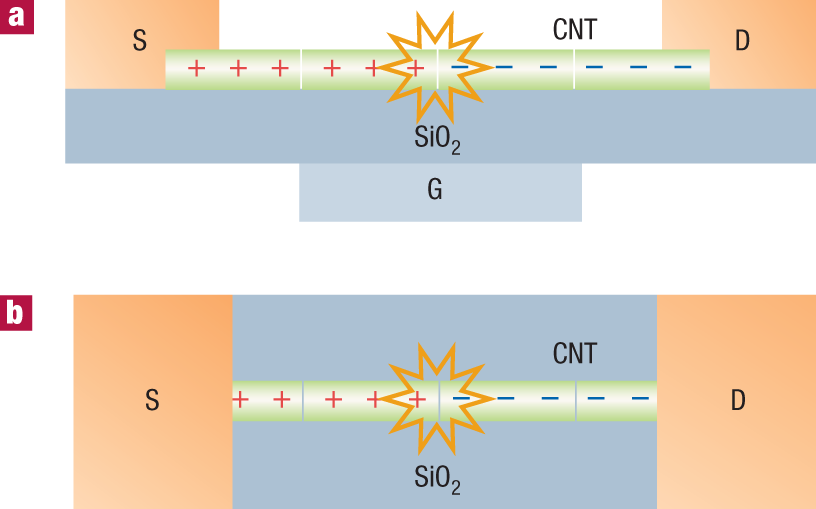
\includegraphics[width=0.6\textwidth]{fig_1}
  \caption{Device structure of a carbon nanotube. (a) Side view. (b) Top view. Infrared emission is generated by the recombination of electrons and holes flowing in the nanotube. Picture from \citet{Muccini}.}
  \label{fig:carbontube}
 \end{center}
\end{figure}

The infrared radiation emitted bu the carbon nanotube FET has some special properties. Due to the elongated shape of the tube, the light is polarised parallel to the tubes axis. This resembles a linearly polarized dipole radiation source. As the bandgap of the nanotube is inversely proportional to its diameter, it is expected that the wavelength can be tuned by changing diameter sizes. Although this is still to be explored, carbon nanotube LETs offer significant potential as nanoscale photon sources that could easily be integrated in optoelectronic devices.

